
\begin{figure}
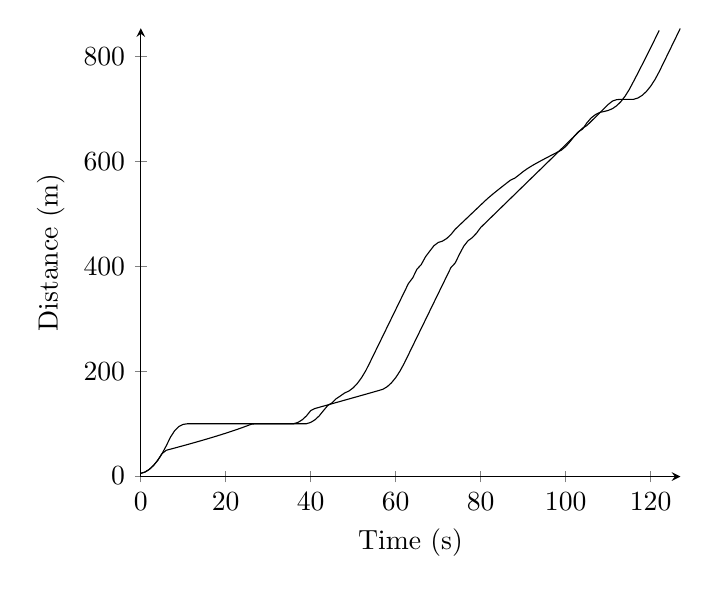
\begin{tikzpicture}
\begin{axis}[
legend style={anchor=west},
axis x line=bottom,
axis y line=left,
ymin=-1,
xlabel=Time (s),
ylabel=Distance (m),
]
\addplot[] coordinates {
(0, 5.1)
(1, 7.6)
(2, 12.6)
(3, 20.1)
(4, 30.1)
(5, 42.6)
(6, 49.1)
(7, 51.2507587657)
(8, 53.4199294455)
(9, 55.6089870099)
(10, 57.8195704245)
(11, 60.0535063982)
(12, 62.3128374321)
(13, 64.5998551155)
(14, 66.9171398634)
(15, 69.2676086146)
(16, 71.6545724347)
(17, 74.0818065376)
(18, 76.5536360003)
(19, 79.0750414808)
(20, 81.6517906672)
(21, 84.2906031573)
(22, 86.9993592384)
(23, 89.7873669902)
(24, 92.6657078557)
(25, 95.647689247)
(26, 98.7494453713)
(27, 99.6521010591)
(28, 99.7196200983)
(29, 99.7196200983)
(30, 99.7196200983)
(31, 99.7196200983)
(32, 99.7196200983)
(33, 99.7196200983)
(34, 99.7196200983)
(35, 99.7196200983)
(36, 99.7196200983)
(37, 99.7196200983)
(38, 99.7196200983)
(39, 99.7196200983)
(40, 102.219620098)
(41, 107.219620098)
(42, 114.719620098)
(43, 124.719620098)
(44, 134.415342321)
(45, 139.378692077)
(46, 147.437449323)
(47, 152.789045989)
(48, 158.436862239)
(49, 162.057551047)
(50, 168.178239854)
(51, 176.798928662)
(52, 187.919617469)
(53, 201.540306277)
(54, 217.660995085)
(55, 234.260995085)
(56, 250.860995085)
(57, 267.460995085)
(58, 284.060995085)
(59, 300.660995085)
(60, 317.260995085)
(61, 333.860995085)
(62, 350.460995085)
(63, 367.060995085)
(64, 377.670995085)
(65, 394.270995085)
(66, 402.960995085)
(67, 417.776786365)
(68, 428.565461431)
(69, 439.071656111)
(70, 445.170421613)
(71, 447.725825791)
(72, 452.781229968)
(73, 460.336634146)
(74, 470.392038324)
(75, 478.09681831)
(76, 485.80197571)
(77, 493.507548215)
(78, 501.213578716)
(79, 508.920116222)
(80, 516.627217001)
(81, 524.334945973)
(82, 531.618257341)
(83, 538.376935676)
(84, 544.903928383)
(85, 551.308130566)
(86, 557.657932451)
(87, 563.975080206)
(88, 567.702311957)
(89, 573.829543707)
(90, 580.383366961)
(91, 586.044317865)
(92, 591.087140943)
(93, 595.74165512)
(94, 600.171919629)
(95, 604.480547833)
(96, 608.726003444)
(97, 612.939651902)
(98, 617.137705502)
(99, 621.328349993)
(100, 628.018994483)
(101, 637.209638974)
(102, 647.515223822)
(103, 656.446279324)
(104, 661.399739379)
(105, 673.313199435)
(106, 682.616096736)
(107, 688.824400137)
(108, 692.990025444)
(109, 694.774298596)
(110, 696.832880678)
(111, 700.245717456)
(112, 705.751147778)
(113, 713.7565781)
(114, 724.262008422)
(115, 737.267438744)
(116, 752.571929318)
(117, 768.203749606)
(118, 784.07687235)
(119, 800.129549454)
(120, 816.3166686)
(121, 832.719090546)
(122, 849.319090546)
};
\addplot[] coordinates {
(0, 5.1)
(1, 7.6)
(2, 12.6)
(3, 20.1)
(4, 30.1)
(5, 42.6)
(6, 57.6)
(7, 74.2)
(8, 86.6997297278)
(9, 94.5649106955)
(10, 98.4573862023)
(11, 99.6094044889)
(12, 99.7189990854)
(13, 99.7189990854)
(14, 99.7189990854)
(15, 99.7189990854)
(16, 99.7189990854)
(17, 99.7189990854)
(18, 99.7189990854)
(19, 99.7189990854)
(20, 99.7189990854)
(21, 99.7189990854)
(22, 99.7189990854)
(23, 99.7189990854)
(24, 99.7189990854)
(25, 99.7189990854)
(26, 99.7189990854)
(27, 99.7189990854)
(28, 99.7189990854)
(29, 99.7189990854)
(30, 99.7189990854)
(31, 99.7189990854)
(32, 99.7189990854)
(33, 99.7189990854)
(34, 99.7189990854)
(35, 99.7189990854)
(36, 99.7189990854)
(37, 102.218999085)
(38, 107.218999085)
(39, 114.718999085)
(40, 124.718999085)
(41, 128.718999085)
(42, 130.991763466)
(43, 133.264934259)
(44, 135.538585572)
(45, 137.812767375)
(46, 140.087651069)
(47, 142.364200289)
(48, 144.641805722)
(49, 146.920748823)
(50, 149.201423132)
(51, 151.484397913)
(52, 153.770532377)
(53, 156.061196958)
(54, 158.358748597)
(55, 160.667717106)
(56, 162.998586851)
(57, 165.387672906)
(58, 170.276758962)
(59, 177.665845018)
(60, 187.554931073)
(61, 199.944017129)
(62, 214.833103185)
(63, 231.433103185)
(64, 248.033103185)
(65, 264.633103185)
(66, 281.233103185)
(67, 297.833103185)
(68, 314.433103185)
(69, 331.033103185)
(70, 347.633103185)
(71, 364.233103185)
(72, 380.833103185)
(73, 397.433103185)
(74, 406.123103185)
(75, 422.723103185)
(76, 437.94674005)
(77, 448.310086877)
(78, 454.285017252)
(79, 462.759947626)
(80, 473.734878001)
(81, 481.62156436)
(82, 489.508620776)
(83, 497.396084253)
(84, 505.283996902)
(85, 513.172406856)
(86, 521.061369382)
(87, 528.950948258)
(88, 536.841217476)
(89, 544.732263378)
(90, 552.62418734)
(91, 560.517109204)
(92, 568.411171684)
(93, 576.306546103)
(94, 584.103439948)
(95, 592.013426484)
(96, 599.923635776)
(97, 607.83410972)
(98, 615.744901439)
(99, 623.656079329)
(100, 631.56773299)
(101, 639.479982156)
(102, 647.39299059)
(103, 655.306988464)
(104, 663.222310055)
(105, 668.1394606)
(106, 676.107993476)
(107, 684.088493134)
(108, 692.08852096)
(109, 700.123987677)
(110, 708.236107629)
(111, 714.641215789)
(112, 717.417627956)
(113, 718.028865702)
(114, 718.059919638)
(115, 718.059919638)
(116, 718.059919638)
(117, 720.559919638)
(118, 725.559919638)
(119, 733.059919638)
(120, 743.059919638)
(121, 755.559919638)
(122, 770.559919638)
(123, 787.159919638)
(124, 803.759919638)
(125, 820.359919638)
(126, 836.959919638)
(127, 853.559919638)
};

\end{axis}
\end{tikzpicture}
\label{tik:100:49}
\caption{100 percent diving with GSC on route $49$}
\end{figure}
